\chapter{Results and Conclusions} \label{results}

The execution time of the original and modified libraries were compared on an NVidia Jetson Nano ARM board. As was already observed by Simone Pistilli in \cite{simonepap} for the JPEG compression algorithm, NanoJPEG CUDA also shows better performance than the original NanoJPEG only above a certain image size, which is roughly 1 Megapixel, YCbCr 4:2:0.

YCbCr 4:4:4 moves the convenience threashold higher, because no upsampling is needed, reducing the opportunities to use GPU time.

Halving of the processing time was observed on a 6000x4000 image on the CUDA version compred to the original.

The process is substantially bound by the disk I/O bandwidth. Using four streams for IDCT allows to copy data to the GPU and to execute the IDCT kernels while the CPU is still reading data from disk, reducing serial time of the operation. The reduction is however far smaller than the theoretical 75\% because in this phase of the algorithm the GPU is under-utilized. An intermediate version of the program with a single CUDA stream for the IDCT showed a time penalty of 23\% compared to the final version with four streams (image: 4272x2848 YCbCr 4:2:0 shown in much smaller form in \autoref{fig:foresta}).

The image size lower threshold discourages the use of this library for consumer products, however future applications could arise that would benefit from the use of dedicated processing power to decompress very high resolution images in real-time, embedded applications, in which case the use of GPGPUs for the purpose would be second only to application specific processors.

\begin{figure}
    \centering
    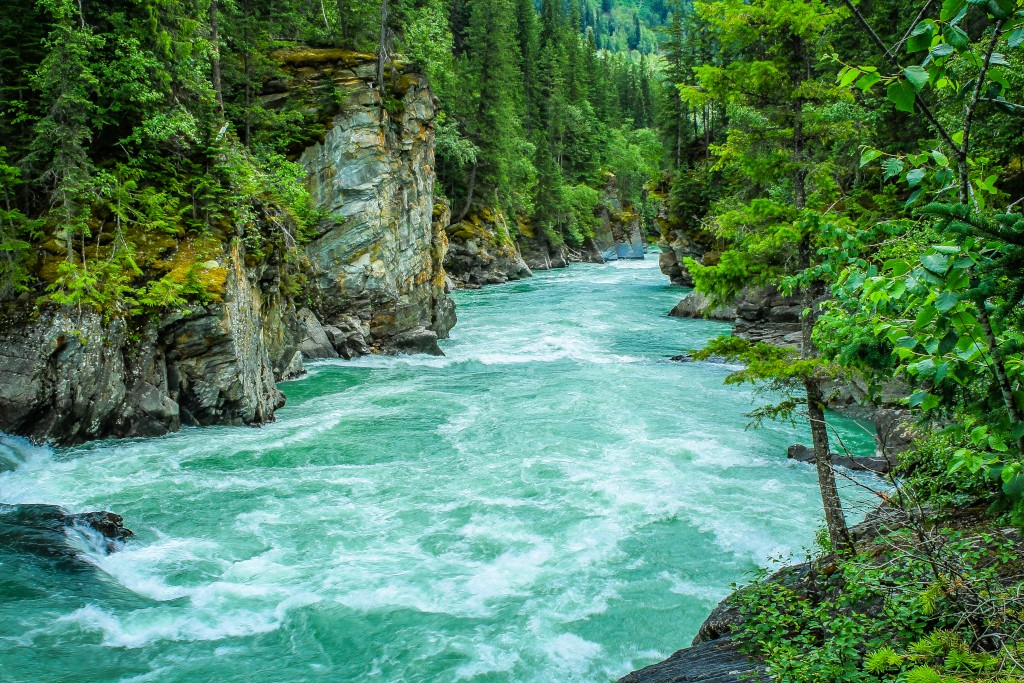
\includegraphics[width=1\textwidth]{Pictures/ph1_small.jpg}
    \caption{Thumbnail of a 4272x2848 pixel, YCbCr 4:2:0 image which in the decompression tests showed a speedup from 3.5s (with the original NanoJPEG), to 2.7s (with one-stream NanoJPEG CUDA), to 2.23s (with final NanoJPEG CUDA)}
    \label{fig:foresta}
\end{figure}
